\documentclass{article}

% ---- Style: official NeurIPS 2026 workshop style if present, otherwise a
% ---- standalone fallback that compiles anywhere.
\IfFileExists{neurips_2026.sty}{%
  \usepackage[preprint]{neurips_2026}%
}{%
  \usepackage[margin=1in]{geometry}%
  \usepackage{times}%
  \usepackage[numbers,sort&compress]{natbib}%
}

\usepackage[utf8]{inputenc}
\usepackage[T1]{fontenc}
\usepackage{graphicx}
\usepackage{booktabs}
\usepackage{amsmath}
\usepackage{xcolor}
\usepackage{url}
\usepackage{microtype}

% Red bracketed marker for the small set of numbers that await a named computation.
\newcommand{\pending}[1]{\textcolor{red}{[\textsc{pending}: #1]}}
\newcommand{\todo}[1]{\textcolor{red}{[TODO: #1]}}

\title{MergeGym: Predicting, Resolving, and Scheduling Around Conflicts Between Concurrent AI Coding Agent Pull Requests}

\author{Anonymous submission}
\date{}

\begin{document}

\maketitle

\begin{abstract}
Autonomous coding agents now open pull requests (PRs) concurrently in the same repositories, yet mainstream software-engineering benchmarks evaluate one agent making one change in isolation, and no benchmark grounded in in-the-wild agent PR streams scores collisions between changes in flight. We introduce \textbf{MergeGym}, a benchmark mined from real agent activity in the wild: 577{,}045 labeled co-active agent-PR pairs (42{,}600 with overlapping changed files, 7.38\%) across 1{,}100 GitHub repositories. % src: verification_log sizes/anatomy
MergeGym defines three tracks. \emph{T1 (interference prediction)}: from PR-open-time text, predict whether two in-flight PRs will touch the same files; on a frozen 5{,}387-pair test set a zero-shot LLM reaches 0.704 AUC and a trained repo-held-out logistic model 0.644, while a filename-extraction baseline (0.574) quantifies how much of the signal is post-hoc file mentions in PR bodies. % src: t1_leaderboard.csv
\emph{T2 (resolution)}: 6{,}387 both-merged conflicting pairs over 391 repositories, released with a documented SHA re-acquisition and replay protocol under which 92.9\% of candidates replay and 21.1\% conflict textually (1{,}252 verified conflicts), with a measured resolution floor: the repository's own reconciliation takes the later PR's side for 49.6\% of conflict hunks; agent-authored concurrent changes are a population the existing human-merge resolution benchmarks do not cover. % src: verification_log sizes
\emph{T3 (scheduling)}: 97 replayed per-repository episodes (19{,}397 PRs) where a policy delays arrivals to de-overlap conflicting pairs; an oracle gate de-overlaps 100\% of labeled overlaps at a median 33.4\% makespan inflation---about $5\times$ cheaper than serializing everything (167.3\%)---and a causally-valid trained gate recovers a median 91.7\% at 65.0\% inflation. % src: t3_summary.json
Conflicts carry measurable cost: the later PR of a conflicting pair shows a within-repository merge-odds ratio of 0.851, an association that survives excluding duplicate-task pairs. % src: mh_robustness.json
MergeGym makes reducing that cost a benchmarked target.
\end{abstract}

\section{Introduction}
\label{sec:intro}

Coding agents have moved from demos to sustained activity on real repositories: the AIDev dataset records 932{,}791 agent-authored PRs on GitHub \citep{li2026aidev,li2025rise}. % src: [aidev]
They increasingly work \emph{at the same time}. Prior work established that 79.4\% of agent PRs in the curated AIDev population are co-active with another agent PR in the same repository, yielding 580{,}913 co-active pairs, and that replaying sampled pairs with \texttt{git merge-tree} produces textual merge conflicts in 19.8\% of intra-agent and 41.7\% of cross-agent overlapping-file pairs \citep{xu2026agentprs}. % src: [xu2026]
AgenticFlict independently measured a 27.67\% PR-versus-mainline conflict rate among the $\sim$107K successfully replayed PRs of a 142{,}652-PR agent corpus \citep{ogenrwot2026agenticflict}. % src: [agenticflict] 142,652 collected / 107K+ replayed / 27.67%
The measurement phase is done. What is missing is a benchmark that turns the interaction between concurrent agent PRs into tasks: no benchmark grounded in real, in-the-wild agent PR streams scores an agent, or a meta-agent orchestrator, on whether its change collides with another change in flight (CooperBench \citep{khatua2026cooperbench} constructs and executes such collisions on synthesized task pairs; \S\ref{sec:related}).

MergeGym\footnote{Name disambiguation: MergeGym is not SWE-Gym \citep{pan2025swegym} (single-agent training environments; 2{,}438 instances) --- though T3 genuinely is a gym-style sequential decision environment, which earns the suffix --- and is unrelated to both MergeBench \citep{mergebench2025llm} (model-parameter merging) and Merge-Bench \citep{schesch2026mergebench} (human-authored conflict hunks).} % src: [swegym] 2,438
fills this gap with three coupled tracks over the same corpus of real co-active agent-PR pairs: \emph{predict} interference at PR-open time (T1), \emph{resolve} the conflicts that materialize (T2), and \emph{schedule} the arrival stream so they never materialize (T3). We say ``concurrent agent PRs'' rather than ``concurrent agents'' deliberately, and we state the corpus composition up front rather than in the limitations: 92.2\% of pairs are Codex--Codex, and two repositories --- \texttt{mochilang/mochi} (369{,}597 pairs) and \texttt{MontrealAI/AGI-Alpha-Agent-v0} (134{,}132) --- hold 87.3\% of all pairs. % src: verification_log anatomy
Today's concurrency is dominated by one platform fanning out PRs in a few hot repositories; cross-agent pairs are a small stratum (0.50\% \citep{xu2026agentprs}) but a far more conflict-prone one: 24.4\% [95\% CI 22.9, 26.0] under our shared-file label, and 41.7\% in prior merge-tree replay \citep{xu2026agentprs}. % src: [xu2026] 0.50%, 41.7%; verification_log 24.42%; p1_headline_cis.json CI
The benchmark is engineered around this skew (per-repository caps, mega-repository exclusions, repository-held-out splits, with/without-mega sensitivity), and we present the skew as a property of the deployment distribution being benchmarked, not a sampling accident.

Interference is not free. The later PR of a conflicting pair merges at 73.3\% versus 86.0\% for non-conflicting pairs; most of that raw gap is compositional, but the repository-stratified Mantel--Haenszel merge-odds ratio is 0.851 (95\% CI [0.825, 0.878]) --- an $\sim$15\% within-repository odds gap, associational rather than causal --- and the association survives excluding near-duplicate-task pairs (\S\ref{sec:data}). % src: verification_log outcomes; mh_robustness.json
Classic evidence adds that conflict-implicated code is roughly twice as bug-prone \citep{brindescu2020emse}. % src: [brindescu]
Meanwhile, coordination methods for concurrent coding agents --- CAID's asynchronous delegation \citep{geng2026caid}, SPOQ's dependency-ordered wave dispatch \citep{spoq2026}, cohesion-aware task partitioning \citep{cohesion2026}, git-native coordination substrates \citep{sarkar2026grite} --- are evaluated on repurposed single-agent benchmarks or bespoke substrates, with no common replay benchmark over in-the-wild agent PR streams to compare them on (\S\ref{sec:related}). CooperBench \citep{khatua2026cooperbench} constructs and executes two-agent tasks with embedded conflicts; MergeGym is complementary --- mined rather than constructed, and the only benchmark with prediction and scheduling tracks (\S\ref{sec:related}).

\paragraph{Contributions.} We make three contributions, machinery first:
\begin{enumerate}
  \item \textbf{The MergeGym benchmark}: three tracks with frozen split manifests, a replay/simulation harness, and a leakage-controlled T1 headroom ladder --- nine uniform baselines from repository base rate (0.601 AUC) through a filename-leakage probe (0.574) and a trained repository-held-out model (0.644) to a zero-shot LLM (0.704) and its metadata-fused ceiling (0.740), with error anatomy showing the residual positives flow through files that PR-open-time text cannot see. % src: t1_leaderboard.csv
  \item \textbf{T3 scheduling episodes with measured Pareto baselines}: 97 per-repository episodes replaying 19{,}397 real PR arrivals, scored as \emph{labeled overlaps de-overlapped} versus throughput lost. FIFO serialization de-overlaps everything at a median 167.3\% makespan inflation; an oracle gate achieves the same at 33.4\%; a causally-valid trained gate traces the frontier between them (Figure~\ref{fig:pareto}) --- to our knowledge the first replay benchmark for conflict-aware scheduling over in-the-wild agent PR streams (grite's released harness \citep{sarkar2026grite} replays streams from agents instrumented with its own coordination substrate; Cassandra \citep{kasi2013cassandra} scheduled human developers' tasks). % src: t3_summary.json
  \item \textbf{T2, a resolution suite over agent-authored concurrent changes}: 6{,}387 both-merged conflicting candidate pairs (391 repositories, 88 cross-agent) with a fully documented construction protocol --- SHA re-acquisition from GitHub, pull-ref fetching with measured survival, merge-tree replay, and reconciliation-based ground truth --- released with candidates, harness, replay results (5{,}936 replayed, 1{,}252 conflicting), and a core pilot with trivial-resolver floors; not the first resolution benchmark \citep{schesch2026mergebench,congra2024,shen2024conflictbench}, and not the first agent-era conflict dataset --- AgenticFlict \citep{ogenrwot2026agenticflict} releases 336K+ PR-versus-mainline conflict regions usable for resolution --- but the first suite over conflicts \emph{between two concurrent agent PRs}, with both-merged, repository-reconciliation ground truth. % src: verification_log sizes; [agenticflict] 336K+ regions
\end{enumerate}

\section{Related work}
\label{sec:related}

\paragraph{Single-agent SWE benchmarks.} SWE-bench and its variants \citep{jimenez2024swebench} evaluate one agent resolving one issue; SWE-Gym \citep{pan2025swegym} and R2E-Gym \citep{r2egym2025} provide executable environments for training such agents. All are single-agent, single-change: none evaluates interactions between concurrent changes. SWE-Gym trains one agent to fix one issue; MergeGym evaluates what happens when many agent PRs edit one repository at once.

\paragraph{Merge conflicts in human collaboration.} Program integration and merging have a long lineage \citep{horwitz1989integrating,mens2002survey}. Workspace-awareness and speculative-merging tools detect conflicts early \citep{sarma2012palantir,brun2011crystal}, and Cassandra scheduled human developers' tasks to minimize conflicts \citep{kasi2013cassandra} --- the direct precedent for T3, at conflict rates of 7.6--19.3\% of merges. % src: [cassandra]
Large-scale studies characterize the structure and life-cycle of conflicts in human merges \citep{ghiotto2020tse,nelson2019lifecycle}.
Prediction from Git features was studied at scale by \citet{owhadi2019predicting} (267{,}657 merge scenarios, 9 light-weight Git feature sets; ESEM 2019), following indicator studies that found lightweight signals largely non-predictive \citep{lessenich2018indicators}. % src: [owhadi] 9 feature sets; [lessenich]
Neural resolution includes MergeBERT \citep{svyatkovskiy2022mergebert} and DeepMerge \citep{dinella2021deepmerge}; benchmarks include ConflictBench (180 Java scenarios) \citep{shen2024conflictbench}, ConGra \citep{congra2024}, and Merge-Bench (7{,}938 hunks over 11 languages; best models resolve under 60\%) \citep{schesch2026mergebench}. % src: [conflictbench][mergebench-conf]
Beyond textual conflicts, semantic-conflict detection uses verification, tests, or static analysis \citep{sousa2018safemerge,dasilva2024semantic,dejesus2023semantic}. All of these are built from human-authored merges; MergeGym's claim for T2 is distribution-first, not task-first.

\paragraph{Agent-era conflict measurement.} AIDev \citep{li2026aidev,li2025rise} provides the substrate; follow-up studies examine rejection outcomes \citep{rejection2026} among others. AgenticFlict \citep{ogenrwot2026agenticflict} measures PR-versus-mainline conflict rates (27.67\%) and releases 336K+ fine-grained conflict regions usable for resolution training and evaluation, but has no PR--PR pairing and no scheduling; \citet{xu2026agentprs} measured co-active pair conflict rates but built no predictive, resolution, or scheduling tasks --- MergeGym supplies them. Duplicated agent tasks are the agent-era analogue of duplicate pull requests \citep{yu2018duppr}, and they matter here both as a T1 label-noise mechanism and as a confounder we control for in the cost analysis. (``Semantic consensus'' work on conflicts between agent \emph{messages} \citep{semcons2026} is unrelated to merge conflicts despite the terminology.)

\paragraph{Constructed concurrent-agent benchmarks.} CooperBench \citep{khatua2026cooperbench} is the closest existing benchmark: 600+ constructed two-agent tasks over 12 libraries grounded in real repositories, with intentionally embedded merge conflicts, execution-based scoring, and a headline $\sim$30\% success drop under cooperation (``curse of coordination''). % src: [cooperbench] 600+ tasks / 12 libraries / ~30%
It is stronger on ground truth (tests run) and weaker on realism (constructed pairs, fixed two-agent setting). MergeGym is the complement: 577{,}045 pairs mined from real agent activity, with prediction (T1) and stream-level scheduling (T3) tracks CooperBench does not have, and CooperBench's own cooperation penalty is motivation for exactly the scheduling MergeGym measures. CooperBench evaluates whether two agents can cooperate on one constructed conflict; T3 evaluates whether a meta-agent scheduler can manage a stream of hundreds of real tasks --- a different unit of analysis: the population of agent PRs sharing a repository rather than a single agent or a single constructed pair.

\paragraph{Coordination methods without a benchmark.} CAID \citep{geng2026caid}, SPOQ \citep{spoq2026}, CoAgent \citep{coagent2026}, cohesion-aware partitioning \citep{cohesion2026}, and industry guidance \citep{cognition2025dont} all manage concurrent agent work; grite \citep{sarkar2026grite} additionally \emph{measures} duplicate-work reduction, though under its own coordination substrate rather than on an external benchmark. Multi-agent SWE frameworks such as MAGIS \citep{tao2024magis} and MetaGPT \citep{hong2024metagpt} coordinate role-specialized agents \emph{within} one change --- orthogonal to the cross-PR concurrency studied here. T3 gives these methods a common, replayable instrument.

\section{Data, construction, and the cost of interference}
\label{sec:data}

\paragraph{Funnel.} From the curated AIDev population (33{,}596 agent PRs, 2{,}807 repositories with over 100 stars \citep{li2026aidev}), prior work extracted 580{,}913 co-active pairs --- two agent PRs in the same repository whose open intervals overlap \citep{xu2026agentprs}. % src: [aidev][xu2026]
Of these, 577{,}045 pairs (99.3\%) have complete changed-file lists for both PRs and form MergeGym's labeled pool: 1{,}100 repositories, 42{,}600 pairs (7.38\%) labeled \emph{conflicting}, meaning the two PRs changed at least one common file path while co-active.\footnote{Of the 580{,}913 co-active pairs, 3{,}868 are dropped for unavailable rows or incomplete changed-file data on at least one side, leaving 577{,}045. The shared-file label was re-verified against per-PR file lists with zero mismatches on the full pool.} % src: verification_log sizes/anatomy
This label is a \emph{proxy}: by the prior replay, roughly 20\% (intra-agent) to 42\% (cross-agent) of overlapping-file pairs produce textual merge conflicts \citep{xu2026agentprs}. We therefore name the T1 task \emph{interference prediction}, reserve ``conflict'' in the strict sense for T2's merge-tree-verified instances, and use ``conflicting pair'' below as shorthand for the shared-file label.

\paragraph{Anatomy that dictates design.} 65.04\% of conflicting pairs share exactly one file (median 1, p90 13). % src: verification_log anatomy
58.76\% involve at least one source-code file; only 33.88\% are pure configuration/docs under the stated file classification. % src: verification_log anatomy
Same-agent pairs conflict at 7.30\% versus 24.42\% [95\% CI 22.88, 26.03] for cross-agent pairs ($n{=}2{,}858$; 95\% CIs for all headline proportions ship with the release); within the diagonal, Codex--Codex sits at 5.60\% ($n{=}532{,}296$) while Devin--Devin reaches 36.38\% ($n{=}19{,}449$) and Copilot--Copilot 21.68\% ($n{=}19{,}360$). % src: verification_log anatomy
The top-10 repositories by conflict count hold 67.62\% of conflicting pairs. % src: verification_log anatomy
Per-pair conflict probability \emph{falls} with concurrency (36.90\% at 2 open PRs down to 3.32\% above 50; 38.93\% to 11.97\% excluding the two mega-repositories) --- we read this dose-response as compositional, not causal: high-fan-out batch workloads are engineered to be file-disjoint, which is precisely the regime T3's schedulers exploit. % src: verification_log anatomy
These facts drive the construction: per-repository caps and repository-held-out splits (concentration), mega-repository exclusion from training pools (skew), and a source-file filter for T2 (config noise).

\paragraph{The cost of interference.} The later-opened PR of a conflicting pair merges at 73.33\% versus 85.96\% in non-conflicting pairs ($-12.63$pp; pair-level OR 0.449; PR-level deduplicated OR 0.588). % src: verification_log outcomes
Most of that raw gap is compositional --- conflict-heavy repositories merge less. The defensible number is the repository-stratified Mantel--Haenszel odds ratio: \textbf{0.851} (95\% CI [0.825, 0.878], 534 strata). % src: mh_robustness.json baseline
Because duplicate-task siblings (agents assigned the same task, redundant later PR closed unmerged) could generate this penalty without any merge-conflict mechanism, we recompute the MH OR excluding the 6{,}937 pairs with normalized-title Jaccard $\geq 0.5$: OR 0.861 [0.834, 0.889] (514 strata); and excluding the 484 pairs with TF-IDF cosine $\geq 0.7$: OR 0.857 [0.830, 0.884] (528 strata). % src: mh_robustness.json
The penalty survives both duplicate-task exclusions essentially unchanged. We stress this is an \emph{association} between the shared-file label and merge outcome within repositories, not a causal estimate; together with the $\sim 2\times$ bug-proneness of conflict-implicated code \citep{brindescu2020emse}, it is the cost signal that justifies benchmarking avoidance.

\begin{table}[t]
\centering
\caption{MergeGym track sizes (frozen manifests). The T1 test set is conflict-enriched; all P@100 numbers in this paper carry that caveat.}
\label{tab:sizes}
\small
\begin{tabular}{llrrl}
\toprule
Split & Unit & Size & Repos & Notes \\
\midrule
Labeled pool & pairs & 577{,}045 & 1{,}100 & 42{,}600 conflicting (7.38\%) \\ % src: verification_log
T1-test (frozen) & pairs & 5{,}387 & 229 & 39.93\% positive (enriched) \\ % src: t1_manifest_summary.json
T1-train & pairs & 24{,}283 & 870 & 32.40\% positive; repo-held-out from test \\ % src: t1_manifest_summary.json
T2-full & pairs & 6{,}387 & 391 & both merged, $\geq$1 shared source file; 88 cross-agent \\ % src: verification_log sizes
T2-core & pairs & 1{,}614 & 264 & both PRs $\leq$1{,}000 changed lines \\ % src: verification_log sizes
T3 episodes & repos & 97 & 97 & 19{,}397 PRs; 38{,}526 conflicting pairs \\ % src: verification_log sizes / t3_summary.json
\bottomrule
\end{tabular}
\end{table}

\section{The MergeGym benchmark}
\label{sec:benchmark}

\subsection{T1: interference prediction from PR-open-time text}
\label{sec:t1}

\textbf{Task.} Given the two PRs' open-time text (title plus body, bodies capped at 1{,}200 characters in the source data; 21.58\% of bodies hit the cap --- a documented benchmark property) and optional metadata (repository, agent, open times), output the probability that the pair is conflicting. % src: verification_log prediction #10
\textbf{Test} is the frozen 5{,}387-pair enriched set (229 repositories, 39.93\% positive). The test set predates the train-pool construction and is defined by its released manifest rather than a regeneration recipe: it was conflict-enriched by oversampling positive pairs relative to the 7.38\% pool rate, it exhausts the co-active pairs of many small repositories (2{,}787 of its 5{,}387 pairs sit in repositories with no non-test pairs remaining --- the reason the repo-base-rate baseline backfills the global rate), and its 229 repositories include one mega-repository, \texttt{MontrealAI/AGI-Alpha-Agent-v0}, which is excluded from every training pool. % src: t1_manifest_summary.json mega_repos_in_test; ev_headroom repo-rate caveat
\textbf{Train} is built from the mega-repository-excluded pool (73{,}316 pairs, 1{,}098 repositories), capped at 200 pairs per repository stratified by label (29{,}470 pairs), then stripped of all pairs in test repositories: \textbf{24{,}283 pairs over 870 repositories at 32.40\% positive}, repository-held-out from test by construction.\footnote{870 rather than $1{,}098-229=869$ because one test repository is a mega-repository already excluded from the pool.} % src: t1_manifest_summary.json
A balanced probe of 2{,}792 pairs (698 per conflict$\times$cross-agent stratum) ships for the cross-agent slice. % src: verification_log sizes
\textbf{Metrics}: AUC, P@100 (always read against the enriched 39.9\%-positive test set, where random ranking scores 0.40), and mean within-repository AUC over the 64 test repositories with $\geq$10 pairs and both classes (4{,}773 pairs). % src: verification_log prediction #7

\textbf{What the text is.} Agent PR bodies are post-hoc change summaries, not pre-assignment task descriptions: by a stated token-level definition (file-like tokens matched exactly, by path suffix, or by basename against the PR's changed files), 31.22\% of the 10{,}774 test-side texts name at least one file the PR actually changed (48.5\% of pairs on at least one side; a curated-extension variant gives 27.9\%, so the rate is definition-dependent within 28--31\%). % src: t1_manifest_summary.json filename_leakage; caveat band
T1 is therefore \emph{prediction from PR-open-time text}, and we quantify the leakage directly with a filename-overlap baseline in the ladder (\S\ref{sec:results-t1}).

\textbf{Leakage rules.} Test repositories are excluded from every training pool in the benchmark, including T3's gating predictor (trained only on non-episode repositories; \S\ref{sec:t3}). The zero-shot LLM row is a single frozen scoring run released verbatim as a per-pair score file with the benchmark: the model received the two PRs' open-time title{+}body strings (the same text-only input every baseline sees) and returned a scalar conflict probability per pair; the row is a fixed reference point, not a rerun recipe. The run used Claude Sonnet, invoked through Claude Code's \texttt{sonnet} alias in headless mode on 2026-08-12 (%% FILL-IN A: exact version string
), scoring ten pairs per call with each task text truncated to 900 characters; prompt and harness are released. % src: llm_scores.csv; t1_manifest_summary.json test_task_text_format
The zero-shot LLM row also carries a contamination caveat: these are public 2024--2025 repositories that plausibly appear in LLM pretraining data. All labels are recoverable from public git history, so we frame the frozen test set as diagnostic rather than anti-cheating, and commit to temporally rolling refreshes from AIDev updates.

\subsection{T2: resolution of agent-authored merge conflicts}
\label{sec:t2}

\textbf{Candidates (released).} Conflicting pairs where both PRs merged and the overlap survives a source-file filter (lockfiles, generated files, \texttt{dist/}, SVGs removed; 16{,}493/575{,}913 file rows, 2.86\%, under the released filter implementation --- the original construction run's slightly different lockfile/\texttt{dist} rule removed 16{,}545, a $\pm$0.01pp sensitivity with identical downstream counts): \textbf{6{,}387 pairs across 391 repositories} (88 cross-agent; 3{,}779 distinct PRs; median 4 shared source files; median PR size 207 changed lines), with a 1{,}614-pair core in which both PRs are $\leq$1{,}000 lines. % src: verification_log sizes
Top languages by pair count, classified by AIDev repository primary language and re-verified from the released candidate list: TypeScript 2{,}030, C\# 1{,}108, JavaScript 645, Python 612, Go 473; the full language and PR-size composition, including the 1{,}000-line core cutoff, is plotted in Figure~\ref{fig:t2comp} (Appendix~\ref{app:composition}). % src: ev_mergegym T2 language breakdown; re-verified from t2_candidates + repo_stats.language
These are concurrent, agent-authored changes --- a population existing human-merge resolution benchmarks do not cover --- where cross-agent pairs conflicted at 41.7\% versus 19.8\% intra-agent in prior replay \citep{xu2026agentprs}.

\textbf{Construction protocol (documented as part of the benchmark).} The corpus stores file paths and texts, not commits, so replay requires re-acquiring per-PR head/base/merge SHAs from the GitHub API (1{,}633 distinct PRs for the core, 3{,}779 for the full set --- computed from the released candidate lists) and fetching pull refs into partial clones; squash-merged heads are not in mainline history and some refs will have been garbage-collected. The protocol therefore includes an explicit SHA-acquisition step with a \emph{measured survival rate reported as a benchmark statistic}, a piloted go/no-go decision before full-scale cloning, and pinned SHAs plus released conflict bundles (license permitting) so the suite survives upstream history rewrites. \texttt{git merge-tree} replay then filters candidates to textually conflicting pairs.

\textbf{Ground truth and metrics.} For each replay-conflicting pair, the reference is the repository's own reconciliation: the shared files' content at the first mainline commit at or after the second merge, \emph{restricted to the conflicted hunk regions} identified by merge-tree (the two merges land close together --- 47.7\% under 24 hours apart, median gap 27.2 hours, computed on the 6{,}387 released candidates with close time as merge-time proxy --- but whole-file snapshots would absorb unrelated churn). % src: recomputed on t2_candidates.csv.gz (6,387 pairs): 47.66% <24h, median 27.21h
We name the metric \emph{agreement with the repository's reconciliation} (hunk exact-match and normalized similarity); it is not execution-based correctness, and no test suites are run in v1 --- pinned SHAs are designed to admit execution-based scoring later, and calibrated LLM-as-judge evaluation against developer resolutions \citep{shen2026javajudge} is a complementary non-execution alternative. \textbf{Replay yield (v1).} We ran the protocol on all 6{,}387 candidates. Head SHAs were re-acquired through \texttt{refs/pull/N/head} rather than the REST API (one \texttt{git fetch} per repository into a blob-less partial clone), which sidesteps API rate limits and squash-merge history loss: pull refs persist on GitHub regardless of merge strategy. Six candidate repositories (447 pairs, 7.0\%) have since become private or been deleted --- 289 of those pairs sit in three \texttt{antiwork/*} Ruby repositories --- and 4 pull refs were missing in reachable repositories, so \textbf{5{,}936 pairs (92.9\%) replayed}; on the core set, 35 pairs were lost to 5 unreachable repositories and no ref was missing (1{,}579/1{,}614, 97.8\%). Three-way \texttt{git merge-tree --write-tree} replay against the pair's merge-base produced a textual conflict in \textbf{1{,}252 of 5{,}936 full pairs (21.1\% [20.1, 22.1])} and \textbf{162 of 1{,}579 core pairs (10.3\% [8.9, 11.9])}; Table~\ref{tab:t2yield} gives survival and yield by language. Yield rises monotonically with PR size (10.3\% for pairs $\leq$1{,}000 lines, 17.0\% at 1--5k, 25.2\% at 5--20k, 34.3\% above 20k) and with the number of shared source files (5.0\% at one shared file, 9.1\% at two, 21.3\% at 3--5, 24.0\% at 6+); the 88 cross-agent pairs conflict at 31.8\% [23.0, 42.1] versus 20.9\% same-agent, the same direction as the prior 747-pair replay. The two mega-repositories contribute 180 candidates and zero conflicts: every one of \texttt{mochilang/mochi}'s 176 pairs modifies the same file on both sides relative to the merge-base and still merges clean, editing disjoint regions --- file overlap is not textual conflict, at scale. The 1{,}252 replay-conflicting pairs form \textbf{T2-verified v1}; the 162 core conflicts are the pilot set.

\textbf{Ground truth and trivial resolvers (core pilot).} The 162 core conflicts contain 579 conflicted files and 1{,}635 content hunks (4 modify/delete). The repository's reconciliation file exists at the first mainline commit at or after the second merge for 98.9\% of hunks, and 89.8\% of hunks (1{,}469) are locatable in it by three-line context anchors on both sides; the remainder are scored as unlocatable rather than dropped silently. Against those 1{,}469 hunks, \emph{taking the later PR's side} matches the reconciliation exactly for \textbf{49.6\%} of hunks (57.0\% at normalized similarity $\geq 0.9$), taking the earlier PR's side for 28.4\%, and concatenating both sides for 12.8\% (Table~\ref{tab:t2pilot}); an oracle choosing the best trivial strategy per hunk reaches 76.2\%, so 23.8\% of hunks need a resolution that is neither side nor their union. Hunk counts are heavy-tailed --- seven pairs hold 1{,}180 of the 1{,}469 hunks --- so we also report the per-pair macro average (later-PR 50.9\%, earlier-PR 38.0\%). That later-PR floor is the number a learned resolver has to beat; the hunk bundle (context, both sides, and the reconciled region for every locatable hunk) is released so that an LLM resolution run is a named computation over a fixed input, and we list it as the v1.1 item rather than report a partial one. %% FILL-IN B: if 07 has run, replace this clause with: ``a zero-shot Claude Sonnet resolver over a 300-hunk stratified pilot (cap 10 hunks per pair) reaches XX.X\% hunk exact-match (XX.X\% at sim$\geq$0.9; per-pair macro XX.X\%) against the later-PR floor of 49.6\% on the same hunks (Table~\ref{tab:t2pilot}).''


\begin{table}[t]
\centering\small
\caption{T2 SHA survival and merge-tree yield by repository primary language (full 6{,}387-candidate set; core-set rows in the released \texttt{t2\_yield\_by\_language.csv}). Survival = share of candidates whose repository is still reachable and whose pull refs were fetched; yield = share of replayed pairs that conflict textually.}
\label{tab:t2yield}
\begin{tabular}{lrrrrr}
\toprule
Language & Candidates & Repos & Replayed (\%) & Conflicting & Yield (\%) \\
\midrule
TypeScript & 2{,}030 & 110 & 1{,}874 (92.3) & 452 & 24.1 \\
C\#        & 1{,}108 & 37  & 1{,}108 (100.0) & 77 & 6.9 \\
JavaScript & 645 & 18 & 645 (100.0) & 142 & 22.0 \\
Python     & 612 & 77 & 608 (99.3) & 130 & 21.4 \\
Go         & 473 & 33 & 473 (100.0) & 96 & 20.3 \\
Ruby       & 438 & 7  & 149 (34.0) & 34 & 22.8 \\
Rust       & 323 & 27 & 323 (100.0) & 136 & 42.1 \\
Dart       & 228 & 5  & 228 (100.0) & 118 & 51.8 \\
Java       & 207 & 17 & 207 (100.0) & 13 & 6.3 \\
Other      & 323 & 60 & 321 (99.4) & 54 & 16.8 \\
\midrule
All (full) & 6{,}387 & 391 & 5{,}936 (92.9) & 1{,}252 & 21.1 \\
Core ($\leq$1{,}000 lines) & 1{,}614 & 264 & 1{,}579 (97.8) & 162 & 10.3 \\
\bottomrule
\end{tabular}
\end{table}

\begin{table}[t]
\centering\small
\caption{T2 core pilot: agreement with the repository's reconciliation on the 1{,}469 locatable conflict hunks from 162 replay-conflicting core pairs. ``Later PR'' = the side of the later-opened PR. Per-pair macro averages hunk exact-match within each of the 129 pairs with $\geq$1 locatable hunk, then across pairs.}
\label{tab:t2pilot}
\begin{tabular}{lrrr}
\toprule
Resolver & Hunk exact (\%) & Hunk sim$\geq$0.9 (\%) & Per-pair macro exact (\%) \\
\midrule
Take earlier PR & 28.4 & 51.3 & 38.0 \\
Take later PR & 49.6 & 57.0 & 50.9 \\
Union (earlier, then later) & 12.8 & 14.1 & 34.1 \\
Union (later, then earlier) & 12.8 & 14.6 & 34.1 \\
Best-of-trivial oracle (per hunk) & 76.2 & --- & --- \\
%% FILL-IN B: uncomment after running 07_t2_llm_resolver_claude_code.py and paste its three printed numbers
%% Zero-shot LLM (Sonnet, 300 hunks, cap 10/pair) & XX.X & XX.X & XX.X \\
\bottomrule
\end{tabular}
\end{table}


\subsection{T3: scheduling episodes over real task streams}
\label{sec:t3}

\textbf{Episode formalism.} An episode is one repository's replayed agent-PR stream --- the stream comprises the repository's PRs that appear in at least one labeled co-active pair: for each PR, an arrival time (observed open), a duration (observed close $-$ open), its open-time text, and a per-repository conflict oracle --- the exact changed-file-set intersection, precomputed over \emph{all} PR pairs so that pairs newly co-scheduled by a policy are also labeled. A policy sees arrivals online (text and repository state only, never file lists or labels) and decides \textsc{start} or \textsc{delay}; delayed PRs keep their durations and shift their whole interval. Two scheduled PRs overlap iff their half-open intervals $[s, s+d)$ intersect with positive length, finishes processed before arrivals at identical timestamps. Pool: the 97 repositories with $\geq$100 co-active pairs and $\geq$20 conflicting pairs (19{,}397 PRs; 563{,}658 pairs; 38{,}526 conflicting), with the top-50 core at a median 95.5 PRs over 72.1 days at mean concurrency 6.9. % src: verification_log sizes / t3_summary.json

\textbf{Censoring.} 778 PRs share the dataset-wide maximum close timestamp (2025-07-30~23:20:55\,UTC) and are right-censored; their durations are capped at the repository's median over non-censored PRs (759 actually shortened). % src: t3_summary.json / t3_assumptions.md
Capped durations are used consistently in \emph{all} policies including the observed baseline, which then materializes \textbf{18{,}071} conflicting overlaps; all avoidance percentages are relative to this capped-observed baseline, not the 38{,}526 labeled pairs. As machinery verification, replaying with uncapped durations reproduces the labeled conflicting-pair count exactly in 97/97 repositories (38{,}526 = 38{,}526). % src: t3_summary.json verification block

\textbf{Metric: labeled overlaps de-overlapped.} The headline score is the percentage of the baseline's conflicting overlaps that no longer overlap under the policy schedule, \emph{net of} conflicting overlaps the policy newly creates (also reported separately); throughput cost is makespan inflation (\%) and added delay in PR-days per PR. We deliberately do not call this ``conflicts prevented'': the simulation assumes (i) de-overlapping a pair removes that pair's conflict --- labels are frozen to the original PR contents, with no model of the delayed agent regenerating its patch on the new base; (ii) durations are fixed under delay; (iii) agents do not react to scheduling. % src: t3_assumptions.md
Under these stated assumptions the score is a \emph{scheduling-feasibility} measure --- the throughput price of de-overlapping the real arrival stream under different gating signals --- and predictor-gated performance is a function of T1-style predictive accuracy \emph{plus} arrival structure. The oracle policy is the explicit upper bound and the observed replay anchors the origin.

\textbf{Policies.} (a) \emph{observed}: start at arrival. (b) \emph{FIFO-serialize}: concurrency 1. (c) \emph{oracle-gated}: start unless a currently \emph{running} PR truly conflicts (file-set oracle); blocked PRs join a FIFO queue re-checked on every finish, skip-ahead allowed. Because the gate keeps the running set mutually conflict-free, the oracle materializes zero conflicts and creates zero new ones --- exactly 100\% by construction; its interest is its cost. (d) \emph{predictor-gated($\tau$)}: same mechanics with a causally-valid predicted probability in place of the oracle, thresholded at nine values of $\tau$ (0.10, 0.15, 0.20, 0.25, 0.30, 0.40, 0.50, 0.65, 0.80), spanning the train-probability 1st--99th percentiles (0.101--0.801). % src: t3_summary.json taus / KEY

\textbf{The predictor} is trained once on the 13{,}387 pairs in non-episode repositories (30.43\% positive) --- a deliberately small, distribution-shifted pool, disclosed as a property of the baseline --- using only decision-time-computable features: TF-IDF cosine of title+body (IDF fit on the 6{,}911 training documents only), title Jaccard, same-agent indicator, and a trailing repository conflict rate computed from the repository's \emph{observed} pair-close record before the current event time (pairs with censored PRs excluded; smoothed with pseudocount 10 toward the pool rate 0.3043). % src: t3_summary.json / t3_assumptions.md
IRLS logistic regression (L2, standardized) attains held-out-fifth AUC \textbf{0.6615} ($n{=}2{,}677$, single seed-0 split; final model refit on all pairs); the trailing rate dominates (single-feature 0.621; standardized weights $[\text{cos}, \text{jac}, \text{same}, \text{trail}] = [0.232, 0.213, 0.004, 0.546]$). % src: t3_summary.json

\section{Baselines and headroom}
\label{sec:results}

\subsection{T1: the headroom ladder}
\label{sec:results-t1}

\begin{table}[t]
\centering
\caption{T1 leaderboard on the frozen 5{,}387-pair test set. P@100 is on the enriched 39.9\%-positive split (random = 0.40) and uses deterministic tie-breaking; within-repo is the mean AUC over the 64 audited repositories with $\geq$10 pairs and both classes. Fused rows use seed-0 5-fold OOF splits ($\pm$0.003 AUC across fold seeds).}
\label{tab:t1}
\small
\begin{tabular}{lccc}
\toprule
Baseline & AUC & P@100 & Within-repo \\
\midrule
Overlap hours & 0.570 & 0.62 & 0.532 \\ % src: t1_leaderboard.csv
Filename-token overlap (count) & 0.574 & 0.65 & 0.546 \\ % src: t1_leaderboard.csv
Repo base rate (non-test pairs) & 0.601 & 1.00 & 0.500 \\ % src: t1_leaderboard.csv
Title Jaccard & 0.629 & 0.89 & 0.626 \\ % src: t1_leaderboard.csv
TF-IDF cosine & 0.644 & 0.82 & 0.659 \\ % src: t1_leaderboard.csv
Trained repo-held-out LR & 0.644 & 0.89 & 0.684 \\ % src: t1_leaderboard.csv
Fused LR (4 features, 5-fold OOF) & 0.676 & 0.97 & 0.657 \\ % src: t1_leaderboard.csv
Zero-shot LLM & 0.704 & 0.96 & 0.743 \\ % src: t1_leaderboard.csv
LLM + all features (5-fold OOF) & 0.740 & 0.99 & 0.738 \\ % src: t1_leaderboard.csv
\bottomrule
\end{tabular}
\end{table}

\begin{figure}[t]
\begin{minipage}[t]{0.48\linewidth}
\centering
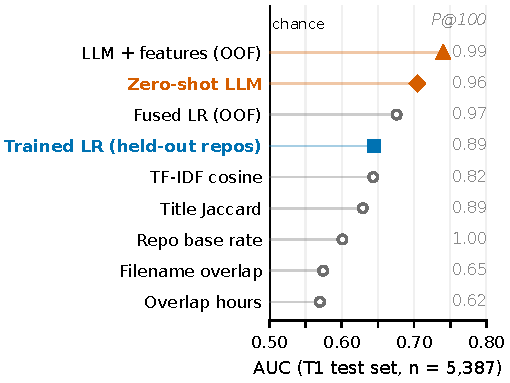
\includegraphics[width=\linewidth]{fig_t1_ladder.pdf}
\caption{The T1 headroom ladder: pooled AUC per baseline (P@100 in the right margin, on the enriched 39.9\%-positive set; random = 0.40). The trained repository-held-out model ties TF-IDF cosine on pooled AUC but has the best within-repository mean after the two LLM rows; the text-only ceiling with metadata fusion is $\approx$0.74.}
\label{fig:ladder}
\end{minipage}\hfill
\begin{minipage}[t]{0.48\linewidth}
\centering
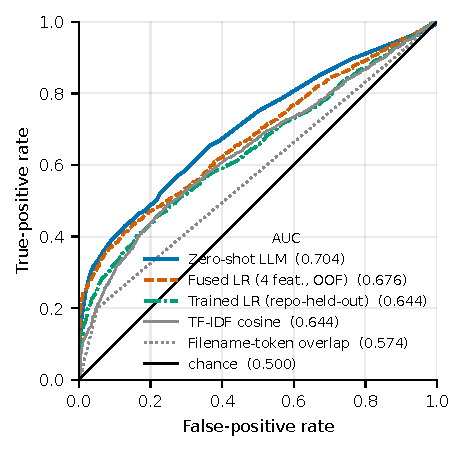
\includegraphics[width=\linewidth]{fig_t1_roc.pdf}
\caption{ROC curves on the frozen T1 test set ($n{=}5{,}387$ pairs; 39.93\% conflicting, 2{,}151 positives). Tie-corrected Mann--Whitney rank AUCs: zero-shot LLM 0.704, fused 4-feature LR (5-fold OOF, seed 0) 0.676, trained repo-held-out LR 0.644 (retrained from the frozen train manifest; reproduces the audited 0.6444 exactly), TF-IDF cosine 0.644, filename-token overlap 0.574, chance 0.500. The two 0.644 rows differ in recipe: the standalone cosine fits IDF on all 10{,}774 test task texts, while the trained LR's TF-IDF feature uses train-fit IDF per the frozen recipe.} % src: figs_extra_p2_checks.json; t1_leaderboard.csv
\label{fig:roc}
\end{minipage}
\end{figure}

Table~\ref{tab:t1} and Figure~\ref{fig:ladder} give nine uniform rows; Figure~\ref{fig:roc} shows the full ROC curves behind the top rows on freshly rebuilt score vectors (released with the benchmark). Three readings matter. \textbf{(1) The honest ceiling of open-time text is $\approx$0.74.} The zero-shot LLM reaches 0.704 pooled AUC (P@100 0.96 on the enriched 39.9\%-positive set; random = 0.40) and adds $+0.065$ over the fused trivial features, which in turn add $+0.036$ on top of it (0.740); repository base rate alone reproduces half the LLM's edge over chance (0.601 vs.\ 0.704), and the fused trivial features reproduce 86\% of it (0.676). % src: t1_leaderboard.csv; ev_headroom; (0.601-0.5)/(0.704-0.5)=0.495, (0.676-0.5)/(0.704-0.5)=0.863
Its within-repository mean (0.743) exceeds its pooled AUC, so the discrimination is not a base-rate artifact; the per-repository breakdown (Figure~\ref{fig:withinrepo}, Appendix~\ref{app:t1quality}) shows AUC above chance in 58 of the 64 audited repositories, and Figure~\ref{fig:t1quality} (Appendix~\ref{app:t1quality}) shows the LLM's probabilities are rank-informative --- precision@$k$ well above the enriched base rate --- while underestimating the conflict rate in the lowest probability bin. % src: t1_leaderboard.csv; figs_extra_p2_checks.json
\textbf{(2) The filename-leakage baseline bounds the post-hoc signal.} Counting shared file-like tokens between the two texts scores 0.574 (a Jaccard variant 0.567; 31.15\% of pairs share $\geq$1 file-like token) --- real but far below the LLM, so most of the LLM's edge is not literal filename extraction, though the disclosure stands: bodies are post-hoc summaries. % src: t1_manifest_summary.json filename_leakage
\textbf{(3) The trained repository-held-out row is the generalization stress test.} A logistic model with TF-IDF cosine, title Jaccard, overlap hours, agent one-hots, and a train-only repository conflict rate reaches 0.644 on test (in-sample 0.821): its strongest feature degenerates to a constant because every test pair sits in an unseen repository, exactly the designed stress --- yet its within-repository mean (0.684) is the best after the LLM rows. The repo-base-rate row's P@100 of 1.00 comes from concentrating picks in high-rate repositories while being exactly 0.500 within-repository --- the cautionary tale the within-repo column exists to expose. % src: t1_manifest_summary.json / t1_leaderboard.csv

\textbf{Error anatomy.} Only 7 label-0 pairs receive LLM probability $\geq$0.9 --- near-duplicate ``sibling'' PRs for the same task that diverged in implementation surface (duplicate PRs in the agent era \citep{yu2018duppr}; arguably semantic near-conflicts the file-overlap label misses). By contrast 468 label-1 pairs (21.8\% of positives) receive $\leq$0.1, dominated by shared CI YAML, \texttt{CHANGELOG}, \texttt{CODEOWNERS}, and agent-instruction files, plus sweeping multi-hundred-file PRs --- overlap invisible in task text by construction. % src: verification_log prediction #8; ev_headroom
File-scope prediction (which files will this task touch?) is T1's stated open problem.

\subsection{T3: the de-overlapping Pareto frontier}
\label{sec:results-t3}

\begin{figure}[t]
\begin{minipage}[t]{0.48\linewidth}
\centering
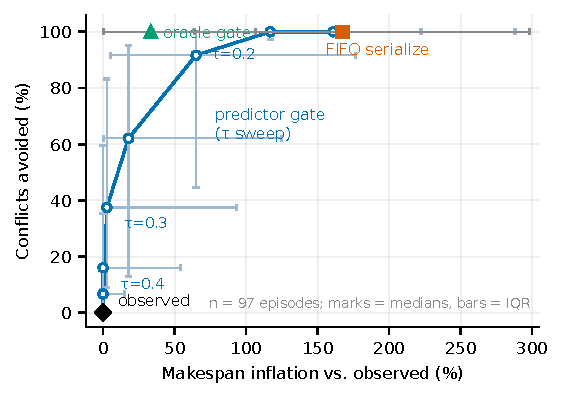
\includegraphics[width=\linewidth]{fig_t3_pareto.pdf}
\caption{T3 frontier over 97 episodes: labeled overlaps de-overlapped (\%, net of newly created overlaps) versus makespan inflation. Marks are medians, bars IQRs. The oracle gate matches FIFO's 100\% at roughly one-fifth the inflation; the trained gate ($\tau$ swept) traces the intermediate frontier, with the observed baseline at the origin ($\tau{=}0.80$ nearly coincides with it).}
\label{fig:pareto}
\end{minipage}\hfill
\begin{minipage}[t]{0.48\linewidth}
\centering
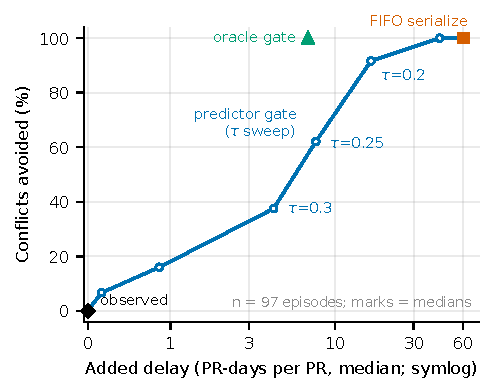
\includegraphics[width=\linewidth]{fig_t3_delaycost.pdf}
\caption{The same frontier with added delay per PR as the cost axis ($n{=}97$ episodes; marks are per-episode medians; net-avoided convention as in Figure~\ref{fig:pareto}). FIFO adds 60.3 PR-days per PR for 100\% avoided; the oracle gate needs 6.9; the predictor gate reaches 91.7\% net avoided at 16.5 ($\tau{=}0.20$), 62.1\% at 7.6 ($\tau{=}0.25$), and 37.5\% at 4.2 ($\tau{=}0.30$), with the observed baseline at $(0,0)$. The $x$-axis is symlog (linear below 1 PR-day/PR).} % src: t3_summary.json; figs_extra_p2_checks.json
\label{fig:delaycost}
\end{minipage}
\end{figure}

\begin{table}[t]
\centering
\caption{T3 policy results. Medians (across 97 episodes) are the headline; pooled columns recompute percentages from summed counts and are dominated by the mega-repositories. De-overlapped \% nets newly created conflicting overlaps; ``new'' reports them separately (pooled totals). The $\tau{=}0.50$ and $\tau{=}0.65$ rows are omitted for space; the full nine-threshold grid ships in the released per-episode results.}
\label{tab:t3}
\small
\begin{tabular}{lrrrrrr}
\toprule
 & \multicolumn{3}{c}{Median over episodes} & \multicolumn{3}{c}{Pooled totals} \\
\cmidrule(lr){2-4}\cmidrule(lr){5-7}
Policy & de-ovl.\,\% & infl.\,\% & delay/PR (d) & de-ovl.\,\% & infl.\,\% & new \\
\midrule
Observed (anchor) & 0.0 & 0.0 & 0.00 & 0.0 & 0.0 & 0 \\ % src: t3_summary.json observed
FIFO-serialize & 100.0 & 167.3 & 60.3 & 100.0 & 280.4 & 0 \\ % src: t3_summary.json fifo
Oracle-gated & 100.0 & 33.4 & 6.9 & 100.0 & 91.6 & 0 \\ % src: t3_summary.json oracle
Predictor $\tau{=}0.10$ & 100.0 & 160.8 & 58.3 & 99.1 & 271.3 & 94 \\ % src: t3_summary.json tau 0.1
Predictor $\tau{=}0.15$ & 100.0 & 116.9 & 43.2 & 91.4 & 228.9 & 623 \\ % src: t3_summary.json tau 0.15
Predictor $\tau{=}0.20$ & 91.7 & 65.0 & 16.5 & 73.7 & 155.6 & 1{,}358 \\ % src: t3_summary.json tau 0.2
Predictor $\tau{=}0.25$ & 62.1 & 17.8 & 7.6 & 53.3 & 109.8 & 2{,}378 \\ % src: t3_summary.json tau 0.25
Predictor $\tau{=}0.30$ & 37.5 & 2.7 & 4.2 & 31.5 & 85.5 & 3{,}951 \\ % src: t3_summary.json tau 0.3
Predictor $\tau{=}0.40$ & 16.0 & 0.0 & 0.9 & 22.6 & 61.2 & 2{,}855 \\ % src: t3_summary.json tau 0.4
Predictor $\tau{=}0.80$ & 0.0 & 0.0 & 0.0 & 4.2 & 8.5 & 761 \\ % src: t3_summary.json tau 0.8
\bottomrule
\end{tabular}
\end{table}

Figure~\ref{fig:pareto} and Table~\ref{tab:t3} are the paper's centerpiece. \textbf{Serializing everything is punitive}: FIFO de-overlaps 100\% of labeled overlaps at a median 167.3\% makespan inflation and 60.3 added PR-days per PR. \textbf{Perfect information is cheap}: the oracle gate achieves the same 100\% (zero materialized, zero newly created --- the gate provably keeps the running set mutually conflict-free) at a median 33.4\% inflation and 6.9 PR-days per PR, about $5\times$ cheaper than FIFO by medians and $19\times$ by pooled added delay (167{,}308 vs.\ 3{,}203{,}635 PR-days); Figure~\ref{fig:delaycost} re-plots the frontier with added delay per PR as the cost axis. % src: t3_summary.json fifo/oracle totals
The gap between FIFO and oracle is the value of knowing \emph{which} pairs interfere --- the quantity T1 predicts.

\textbf{An imperfect predictor buys most of it.} The trained gate (held-out AUC 0.6615) interpolates monotonically across the nine thresholds from do-nothing ($\tau{=}0.80$: median 0\% at 0\% inflation) to near-FIFO ($\tau{=}0.10$: 100\% at 160.8\% inflation), with a usable knee at $\tau{=}0.20$ (median 91.7\% de-overlapped at 65.0\% inflation) and $\tau{=}0.25$ (62.1\% at 17.8\%); the per-episode dispersion behind the knee medians, and the diversity of the 97 episodes themselves, are shown in Figure~\ref{fig:episodes} (Appendix~\ref{app:composition}). % src: t3_summary.json
Newly created overlaps --- pairs the policy pushes into co-activity that were not co-active in the baseline --- peak at 3{,}951 pooled at $\tau{=}0.30$ and are netted out of every de-overlapped figure. % src: t3_summary.json
The remaining oracle-to-predictor gap at matched cost is T3's headroom, and it is exactly what better T1 models (file-scope prediction above all) should close.

\textbf{Sensitivity.} Excluding the two mega-repositories (95 episodes) leaves the medians essentially unchanged (oracle inflation still 33.4\%); the pooled $\tau{=}0.20$ de-overlapped rate \emph{rises} from 73.7\% to 84.0\%, because the censoring-degenerate baseline of the AGI-Alpha repository (6 capped-observed conflicts against 13{,}644 labeled pairs) drops out of the pooled denominator. % src: t3_summary.json sensitivity / t3_assumptions.md
The no-mega variant of Figure~\ref{fig:pareto} is in Appendix~\ref{app:sensitivity}.

\subsection{T2: verified subset and resolution floor}
T2 ships as candidates, protocol, harness, and a first verified subset: 92.9\% of candidates replayed, 21.1\% of them conflict textually (1{,}252 pairs; 10.3\% on the core set), and yield scales with PR size and shared-file count (\S\ref{sec:t2}, Table~\ref{tab:t2yield}). On the 162 core conflicts, the repository's own reconciliation sides with the later PR for half of all conflict hunks and needs genuine synthesis for a quarter (Table~\ref{tab:t2pilot}); that 49.6\% later-PR floor is the bar for learned resolvers. We make no comparability claim against Merge-Bench's under-60\% on human-authored hunks \citep{schesch2026mergebench}; the distributions differ by construction.

\section{Discussion, limitations, and release}
\label{sec:discussion}

\paragraph{``So what --- conflicts are cheap.''} Four answers. (a) They are not config noise: 58.76\% of conflicting pairs touch source code. % src: verification_log anatomy
(b) They are associated with real cost: the within-repository MH merge-odds ratio of 0.851 survives duplicate-task exclusions (\S\ref{sec:data}), and conflict-implicated code is $\sim 2\times$ as bug-prone \citep{brindescu2020emse}. (c) Cross-agent pairs are 0.50\% of volume today but conflict at 24.4\% (41.7\% in strict replay), and multi-agent, multi-vendor deployment is the industry's stated direction with no evaluation standard \citep{geng2026caid,cognition2025dont}. (d) CooperBench's constructed setting independently finds a $\sim$30\% cooperation penalty \citep{khatua2026cooperbench} --- the cost exists even when the ground truth is executable.

\paragraph{Limitations.} T1's label is shared-changed-file interference, a proxy for textual conflict (anchored to prior 747-pair merge-tree replay rates \citep{xu2026agentprs}) that misses semantic conflicts --- the 7 high-confidence false-positive siblings are exhibits; renames are not tracked. T3 is replay, not intervention: the de-overlapping metric is a scheduling-feasibility measure under stated assumptions (frozen labels, fixed durations, no behavioral response), the observed baseline is capped-censored (avoidance measured against 18{,}071 baseline overlaps, not 38{,}526 labeled pairs), and 32/97 repositories are unaffected by capping while censoring-heavy ones lose baseline conflicts. The T3 predictor's training pool is small and distribution-shifted (13{,}387 pairs, 30.4\% positive, non-episode repositories). The corpus skew is disclosed in \S\ref{sec:intro} and engineered around, but cross-agent results remain a small, high-conflict-rate stratum motivating future collection, not the evaluated regime. T2's ground truth is agreement with the repository's own reconciliation --- frequently the same platform rebasing its own PR --- not execution-verified correctness, and its 49.6\% later-PR floor partly reflects exactly that rebase-on-top workflow; 7.1\% of candidates are already unreachable upstream, which is why pinned SHAs and conflict bundles ship with the release. Body truncation (21.58\% at 1{,}200 characters) bounds text-side information.

\paragraph{Ethics and licensing.} All data derive from public GitHub activity in repositories with $\geq$101 stars (median 644; 41.1\% $\geq$1{,}000), redistributed under AIDev's release \citep{li2026aidev}; PR text is public and no personal data beyond public developer activity is processed. % src: verification_log sizes repo_stats
A per-repository license audit accompanies the release; T2 conflict bundles are released only for permissively licensed repositories, with metadata-only fallback otherwise.

\paragraph{Reproducibility.} We release the split manifests (T1 train/test/balanced, T2 full/core candidate lists, 97 T3 episode files), the replay simulator and gating harness, all baseline code (pure-numpy AUC/logistic implementations), per-episode results (97 episodes $\times$ 12 policy/threshold settings), and the datasheet documenting every convention in this paper (censoring rule, overlap definition, tokenizers, tie-breaking). Every number above is traceable to a released artifact; T2's pending numbers are named computations in the released protocol, not claims.


\section{Conclusion}
Concurrent agent PRs are no longer an edge case: four in five agent PRs in AIDev are co-active with another, and the interference between them has been measured but never benchmarked. MergeGym turns that interaction into three tasks over one corpus of 577{,}045 real co-active pairs. T1 shows that PR-open-time text carries real but bounded signal about interference (zero-shot LLM 0.704 AUC, 0.740 fused; filename leakage explains little of it) and that the misses concentrate in files no task description names. T3 shows that the value of that signal is concrete: perfect knowledge of which pairs interfere de-overlaps every conflicting pair at one-fifth the throughput cost of serialization, and a weak trained gate already recovers most of it. T2 supplies the population of agent-authored concurrent conflicts that no resolution benchmark covers --- 1{,}252 replay-verified conflicts, with a measured floor showing the repository sides with the later PR for half of all hunks and needs real synthesis for a quarter. The three tracks share one headroom: predicting which files a task will touch. Closing it improves T1 directly, moves T3's predictor gate toward the oracle, and shrinks the conflicts T2 has to resolve. We release the manifests, harness, replay results, and every number's derivation so that the next coordination method for concurrent coding agents has something to be measured against.

\bibliographystyle{plainnat}
\bibliography{references}

\appendix
\clearpage

\section{T3 sensitivity: excluding the mega-repositories}
\label{app:sensitivity}

\begin{figure}[h]
\centering
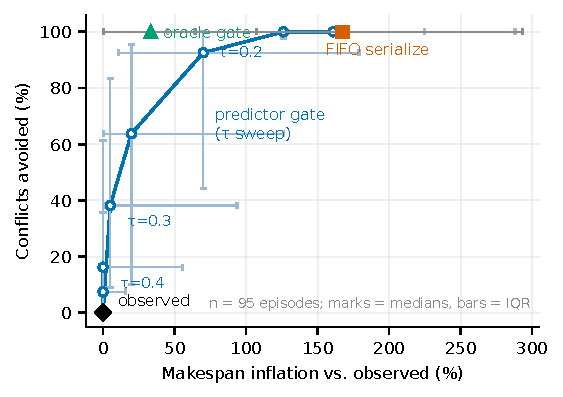
\includegraphics[width=0.62\linewidth]{fig_t3_pareto_nomega.pdf}
\caption{The Figure~\ref{fig:pareto} frontier recomputed over the 95 episodes excluding \texttt{mochilang/mochi} and \texttt{MontrealAI/AGI-Alpha-Agent-v0}. Medians are essentially unchanged (oracle 33.4\% inflation; FIFO 167.3\%); pooled de-overlapped rates rise (e.g., $\tau{=}0.20$: 73.7\% $\to$ 84.0\%) because the censoring-degenerate mega-repository baseline leaves the pooled denominator.} % src: t3_summary.json sensitivity
\label{fig:pareto-nomega}
\end{figure}

\clearpage
\section{T1 probability quality and generalization}
\label{app:t1quality}

Figure~\ref{fig:t1quality} examines the zero-shot LLM's scores as probabilities rather than ranks, and Figure~\ref{fig:withinrepo} breaks its discrimination down by repository; both are referenced from \S\ref{sec:results-t1}.

\begin{figure}[h]
\centering
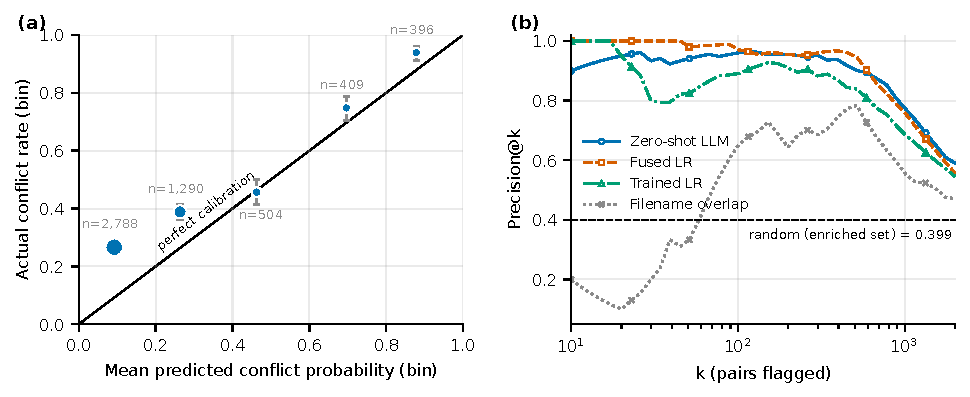
\includegraphics[width=\linewidth]{fig_t1_quality.pdf}
\caption{Zero-shot LLM probability quality on the frozen 5{,}387-pair test set. \textbf{(a)} Reliability diagram over five left-closed probability bins $[0,.2)$, $[.2,.4)$, $[.4,.6)$, $[.6,.8)$, $[.8,1]$: bin counts $n = 2{,}788$/$1{,}290$/$504$/$409$/$396$; mean predicted probability 0.092/0.263/0.463/0.696/0.878 versus actual conflict rate 0.266/0.388/0.456/0.748/0.939; error bars are 95\% Wilson intervals; point size scales with bin count. The upper bins are close to calibrated while the lowest bin substantially underestimates the (enrichment-inflated) conflict rate. \textbf{(b)} Precision@$k$ for $k = 10$--$2{,}000$ (log $x$) against the enriched-set base rate 0.3993 (dashed): LLM P@50 $=$ 0.94 and P@100 $=$ 0.96 under a deterministic descending stable sort (P@50 is tie-sensitive: $\approx$0.958 under random tie-breaking); filename-token overlap P@10 $=$ 0.20 --- its top-count pairs are mostly non-conflicts.} % src: figs_extra_p2_checks.json; verification_log prediction
\label{fig:t1quality}
\end{figure}

\begin{figure}[h]
\centering
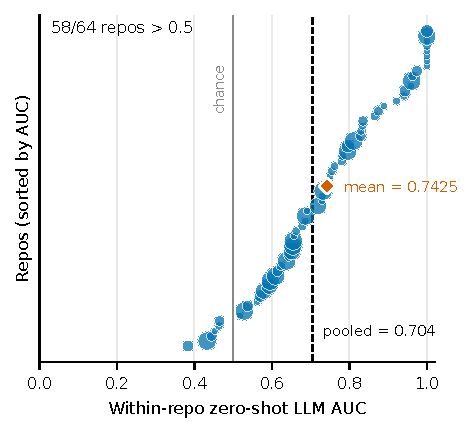
\includegraphics[width=0.62\linewidth]{fig_t1_withinrepo.pdf}
\caption{Per-repository zero-shot LLM AUC over the 64 test repositories with $\geq$10 test pairs and both classes (covering 4{,}773 of the 5{,}387 test pairs; point size scales with per-repository test-pair count). Mean per-repository AUC 0.7425 (diamond); AUC $>$ 0.5 in 58/64 repositories; pooled test-set AUC 0.704 (black dashed line); chance 0.5 (gray line). AUCs are tie-corrected rank AUCs.} % src: figs_extra_p2_checks.json; t1_leaderboard.csv within-repo audit
\label{fig:withinrepo}
\end{figure}

\clearpage
\section{Episode and T2 composition}
\label{app:composition}

Figure~\ref{fig:episodes} characterizes the 97 T3 episodes and the per-episode heterogeneity behind the $\tau{=}0.20$ knee medians quoted in \S\ref{sec:results-t3}; Figure~\ref{fig:t2comp} gives the language and PR-size anatomy of the T2 candidate suite described in \S\ref{sec:t2}.

\begin{figure}[h]
\centering
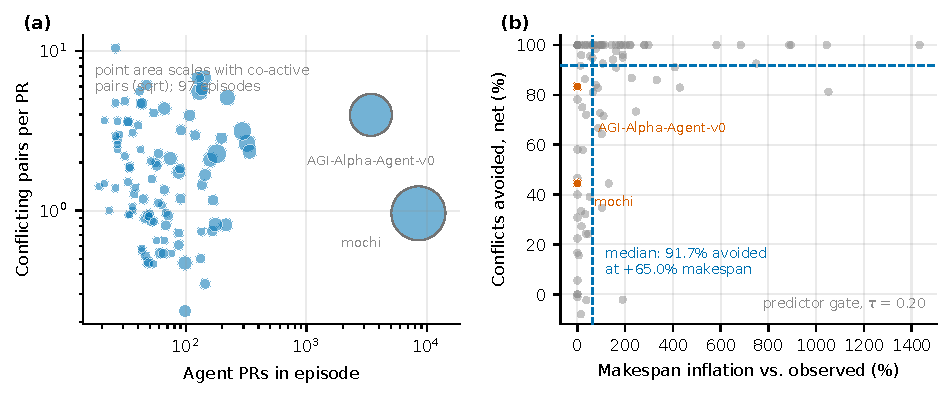
\includegraphics[width=\linewidth]{fig_t3_episodes.pdf}
\caption{\textbf{(a)} The 97 T3 episodes (repositories with $\geq$100 co-active pairs and $\geq$20 conflicting pairs), jointly containing 19{,}397 distinct agent PRs and 38{,}526 labeled conflicting pairs: agent PRs per episode versus labeled conflicting pairs per PR (log--log). Point \emph{area} scales with the square root of co-active pairs (linear-area scaling makes the mega-repositories unplottable); \texttt{mochilang/mochi} (369{,}597 co-active pairs) and \texttt{MontrealAI/AGI-Alpha-Agent-v0} (134{,}132) annotated. Episode PR count is the number of distinct PRs appearing in that repository's labeled pairs. \textbf{(b)} Per-episode makespan inflation versus net conflicts avoided under the predictor gate at $\tau = 0.20$, same 97 episodes; the crosshair marks the per-episode medians, 91.7\% net avoided at $+$65.0\% inflation. ``Net'' $=$ (observed conflicts $-$ conflicts under policy, including newly created ones)$/$observed, and can be negative.} % src: t3_summary.json; figs_extra_p2_checks.json
\label{fig:episodes}
\end{figure}

\begin{figure}[h]
\centering
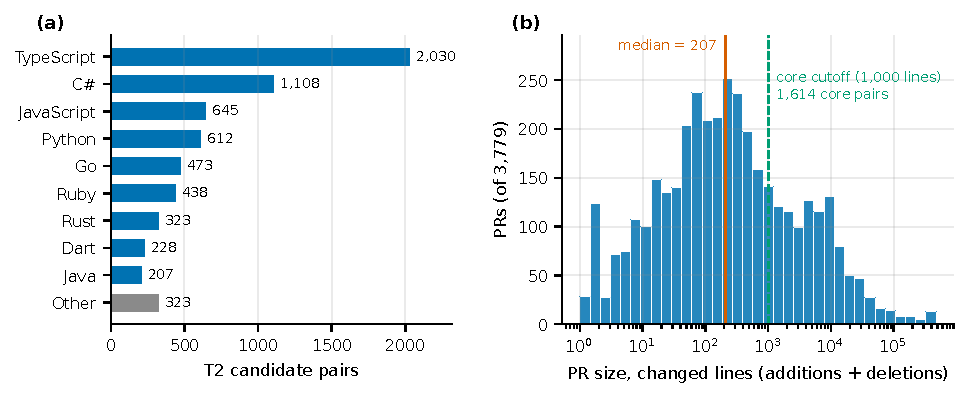
\includegraphics[width=\linewidth]{fig_t2_composition.pdf}
\caption{T2 candidate anatomy: 6{,}387 candidate pairs across 391 repositories (both PRs merged, $\geq$1 shared source file). \textbf{(a)} Candidate pairs by repository primary language (AIDev \texttt{repo\_stats} classification): TypeScript 2{,}030; C\# 1{,}108; JavaScript 645; Python 612; Go 473; Ruby 438; Rust 323; Dart 228; Java 207; Other 323. \textbf{(b)} Per-PR total changed lines (additions $+$ deletions over \emph{all} file rows, not only source files) for the 3{,}779 distinct T2 PRs, log $x$, sizes clipped to $\geq$1 line: median 207 changed lines; the T2-core cutoff (both PRs $\leq$1{,}000 lines, dashed) yields 1{,}614 core pairs.} % src: figs_extra_p2_checks.json; verification_log sizes
\label{fig:t2comp}
\end{figure}

\clearpage
\section{Additional T3 protocol details}
\label{app:t3-details}

Conflict oracle: exact file-path-set intersection from per-PR changed-file lists, applied to all PR pairs including ones never co-active in reality; renames and semantic conflicts are out of scope. % src: t3_assumptions.md
Censoring fill value: 778 PRs carry the dataset-wide maximum close timestamp; caps applied as $\min(\text{duration}, \text{repo median over non-censored PRs})$; no repository needed the global-median fallback. % src: t3_summary.json
Gate mechanics: candidates are checked only against \emph{running} PRs; the FIFO queue is re-scanned on every finish; skip-ahead is allowed, and PRs started during a scan immediately count as running for later PRs in the same scan. % src: t3_assumptions.md
Predictor scoring at simulation time uses the repository's observed historical pair-close record (never the simulated schedule) for the trailing conflict rate; static pairwise logits are precomputed in float32 ($\sim$$10^{-3}$ logit rounding, negligible against the $\tau$ grid). % src: t3_assumptions.md
The full per-episode results table (97 episodes $\times$ 12 policy/threshold rows) ships with the release.

\end{document}
